%   %   %   %   %   %   %   %   %   %   %   %
%   For the final document:
%       > add option 'final' to \documentclass.
%       > change \thedate to \today in groupproject.sty
%       > change option draft=true to draft=false or final=true for package 'minted' in groupproject.sty
%   This will allow listings to render in colour and will ensure todos and draft markings are hidden
%   %   %   %   %   %   %   %   %   %   %   %


\documentclass[a4paper,11pt,twoside,openright]{report}
\usepackage{groupproject}
\usepackage{groupreport}

\begin{document}
%Title page and table of contents
    \pagestyle{plain}
\pagenumbering{roman}

\begin{titlepage}
    \centering
    %\includegraphics[width=0.15\textwidth]{example-image-1x1}\par\vspace{1cm}
    {\scshape\LARGE University College London \par}
    \vspace{1cm}
    {\scshape PHAS3441 group project\par}
    {\scshape Group 5:~\teamname\par}
    \vspace{1.5cm}
    {\huge\bfseries \towrite{\hfill DRAFT COPY \hfill :??} \projectTitle\par}
    \vspace{2cm}
    {\Large\itshape Alexander Goodsell, Lorenzo Foglianti Spadini, Ashleigh Hyslop,\\ Arunyan Kallaivannan, Robert Kent, Calvin Lau, Alan Rutley,\\ Samuel Searles-Bryant, Samuel Wright, Luke Yeo\par}
    \vfill
    Board member:\par
    Dr.~Martin \textsc{Fry}

    \vfill

% Bottom of the page
    {\large \thedate\par}
\end{titlepage}

{\centering
{\itshape \teamname~was chaired by Alexander Goodsell.\par}
\vfill
{\itshape This report was compiled and edited by Samuel Searles-Bryant. Each section is labelled with its original author(s).\par}
\vfill
}

\cleardoublepage

\tableofcontents

    \todo[inline]{Ask MF: would we usually put data sheets for components (motors \emph{etc.}) in the appendix?}
\cleardoublepage
\todototoc
\listoftodos
\cleardoublepage

%Executive summary
    \fancyhead[RO]{Acknowledgements}
\begin{centering}
\chapter*{}\label{acknowledgements}
\addcontentsline{toc}{chapter}{Acknowledgements}
{\Huge \textbf{Acknowledgements}}

\vspace{1.5cm}

The group would like to thank \dots \todo[inline,size=\normalsize,color={red!100!green!33}]{Write acknowledgements}

Martin\\
Lab staff\\
Bartlett

\end{centering}

\cleardoublepage
\pagestyle{fancy}
    \fancyhead[RO]{Executive Summary}
% There is general agreement on the structure of an executive summary - books and training courses emphasize similar points. Typically, an executive summary will:
%
% be approximately 5-10% of the length of the main report
% be written in language appropriate for the target audience
% consist of short, concise paragraphs
% begin with a summary
% be written in the same order as the main report
% only include material present in the main report
% make recommendations
% provide a justification
% have a conclusion
% be readable separately from the main report
% sometimes summarize more than one document
% ---from Wikipedia

% An Executive Summary of not more than 2 A4 pages. This should convey briefly, but precisely, an overall summary of the project, including aims and objectives, the work done, and the final outcome(s). It should be written in such a way as to convince the busy MD of Physics Innovations (UCL) that you have delivered the goods. Remember that in real life, the Executive Summary is often the most important part of a report in leading to the crucial decision. It must, however, be fully backed up by the more extensive detailed material in the body of your report.
% ---from Bartlett's guidance

\chapter*{Executive Summary}\label{executive summary}
\addcontentsline{toc}{chapter}{Executive Summary}
\towrite{Executive summary}

\myBlindSection{Introduction}{writer TBA}


\myBlindSection{Design}{writer TBA}


\myBlindSection{Conclusion}{writer TBA}


%Sections of report
\cleardoublepage
\fancyhead[RO]{\chaptertype~\thechapter: \small\nameref{section \thechapter}}
\glsresetall
\pagenumbering{arabic}
    \chapter{Introduction and Preliminary Research}\label{introduction,research}\label{section \thechapter}

\mySection{Project brief}{writer TBA}\label{project brief}
\towrite{project brief}

\mySection{Art review}{\AH, \AR}\label{art review}
    \begin{figure}%{I}{0.45\textwidth}
        % \vspace{-11pt}
        \centering
        \begin{subfigure}[b]{0.45\textwidth}
            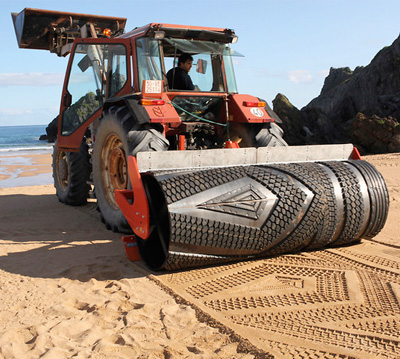
\includegraphics[width=\textwidth]{Files/sand_machine.jpg}
            \caption{Sand-printing tractor. The roller on the front produces the imprints.}
            \label{fig: sand machine}
        \end{subfigure}
        ~
        \begin{subfigure}[b]{0.45\textwidth}
            
\includegraphics[width=\textwidth]{Files/sand_machine_art.jpg}
            \caption{Large-scale imprints produced using the tractor.}
            \label{fig: sand machine art}
        \end{subfigure}
        \caption{Gunilla Klingberg's `sand machine' and the pattern it produces. \small (Retrieved from     \citen{ShiMin2013} on 2016--01--20)}
        \label{fig: sand machine and art}
        % \vspace{-20pt}
    \end{figure}
    Land art (or Earth art) utilizes the landscape itself to produce the art. Structures are often made by placing natural materials, such as rocks or twigs, onto the land to form a pattern or picture. Another way they are produced is by sculpting the land to form patterns. The art is not simply placed onto the land, rather the land is the means of the creation. Pieces are often ephemeral in nature, being left to erode due to natural conditions over time, and so now only exist in photographic and video documentation.\\
    A significant inspiration for the creation of land art came from people's awareness of the negative impact they can have on the environment around them. By incorporating art into the natural landscape, artists hope that it will change people’s perspective of the environment around them.

    Land art is a largely American movement which began in the late 1960s. The movement is an offshoot of conceptualism and minimalism and was a protest to the commercialization of American art, leading the artists to produce works which were removed from the art market.\\
    It can be argued that land art was created by ancient cultures. Examples of land art occur around the world, such as the Nazca lines produced by the Nazca in southern Peru and The Great Serpent Mound in Ohio, US. It is believed that these pieces could have been created as a form of worship to the gods of the cultures which made these pieces.\\
    The modern movement began with the group exhibition ``Earth works'' in New York City in October 1968. In the following year, Willoughby Sharp curated the ``Earth Art'' exhibition at Cornell University which included many artists, such as Robert Smithson and Richard Long, who were big influences within the movement. Due to their monumental size the pieces were usually documented in photographs and maps which the artist could exhibit in a gallery. Land art was occasionally also produced within galleries; this was done by bringing in materials from the landscape and using them to create installations.\\
    %One of the most well-known artists in this movement was Robert Smithson. His best known piece, and possibly the most famous example of land art, is “Spiral Jetty” which was constructed in April 1970. It was constructed at Rozel Point, Great Salt Lake, Utah, reportedly this location was chosen by Smithson due to the blood red colour of the water which submerges the art at times of normal precipitation (the jetty is revealed during times of drought). The spiral structure was constructed using 6650 tons of black basalt rocks which were transported and manipulated in the lake bed using dumper trucks, tractors and front end loaders. The construction was documented and presented as a film, also called Spiral Jetty [3].


    \subsection{Sand art}\label{sand art}
        \begin{wrapfigure}{I}{0.45\textwidth}
            % \vspace{-11pt}
            \centering
            \begin{subfigure}[b]{0.45\textwidth}
                
\includegraphics[width=\textwidth]{Files/andres_amador.jpg}
                \caption{Andres Amador using a rake to produce his playa pictures.}
                \label{fig: andres amador}
            \end{subfigure}
            \begin{subfigure}[b]{0.45\textwidth}
                
\includegraphics[width=\textwidth]{Files/andres_amador_art.jpg}
                \caption{Large-scale imprints produced using the tractor.}
                \label{fig: andres amador art}
            \end{subfigure}
            \caption{\small (Retrieved from \citen{andresamador} on 2016--01--23)}
            \label{fig: andres amador and art}
            % \vspace{-20pt}
        \end{wrapfigure}
        There are various styles of sand art; the main two are large scale sculptures and 2-dimensional freehand drawings. Over recent years smaller scale sand storytelling has developed which is concerned with both the performance and the final images produced. Large-scale artists mostly use easily accessible equipment such as shovels, buckets and rakes for freehand drawing and trowels and spatulas for sculpting. However, Swedish artist Gunilla Klingberg has developed a sand-printing tractor(Figure~\ref{fig: sand machine}), which produces large imprints across beaches (Figure~\ref{fig: sand machine art}). A low tide is needed for both printing and free hand drawing due to the wet sand.\\
        Jim Denevan, a popular freehand sand artist, ranges the scale of his work from small beach compositions to land works the size of a city. He has done live performances for exhibitions at Yerba Buena Centre for the Arts, 2005, and the Vancouver Sculpture Biennale, 2010. His work has also been featured in popular magazines such as the New York Times Magazine and National Geographic. Denevan does not use any sort of measuring tools and spends an average of 7 hours, walking about 30 miles, when producing his work. After all of this time his work is soon washed away by the incoming tide.\\
        Though the transient nature of this art form seems defeatist, it is actually the motivation for many sand artists. Andres Amador says he prefers a temporary medium and is much more concerned with his ``process and less about the result.'' He does not produce any form of permanent art work. Mr Amador's pieces, known as playa paintings, are produced using simply a rake and a rope as a guide (Figure~\ref{fig: andres amador and art}).

        Charlene Lanzel produces small-scale sand stories. Their creation can be observed as she creates images on a table top, projected onto a large screen sitting above her. Lanzel produces her images in darkness, the sand sitting on a glass table with lights underneath. Unlike other forms of sand art, her work is not washed away by the tide; instead she destroys the work herself in order to produce fluid images that play like an animation. Lanzel uses soundtracks alongside her performance to tell her stories and fully immerse her audience.

        Sand sculpture may be the largest scale form of sand art. Competitions are popular on beaches around the world and sculptures with the stature and solidity of woodcarvings are often produced.  Sculpture is also the most permanent style: many sculptures produced indoors last for more than a year.

\mySection{History of robotics}{\SW, \AK}\label{history of robotics}
    Autonomous robots have become common in many fields: factories make use of autonomous workers; space exploration vehicles include autonomous navigation systems and automated scientific instruments; military and commercial aircraft use autonomous systems to stay airborne; and large utilities providers (\eg water treatment plants and power stations) have some automated control systems.\\
    These technologies have been developing since the early 20th century. Some of those developments are of particular interest with regard to the development of a sand art--drawing robot.

    One difficult challenge in autonomous robotics is that of navigation. Many of the most advanced navigating robots that have been designed have been entrants in a Micromouse competition.\\
    The model of the Micromouse competition was introduced in 1977 by IEEE Spectrum magazine.\cite{harrison2010} It involves robots competing to get to the centre of a maze in the fastest time. There have been many variations of the rules, but the main theme is that the robots are autonomous. The inaugural competition was held in 1979 and was won by a high-speed dumb wall follower. In 1980 an entrant became the first Micromouse robot to find the centre of the maze and know it had done so, although it travelled at only \SI{0.2}{\meter\per\second}.

    Autonomous movement presents several other challenges. Many robots have been developed to move over different terrains. In particular these have been used to explore the surface of alien planets.\\
    The history of successful Mars rover missions began in 1997 with NASA's pathfinder mission. The `Pathfinder' lander contained a rover, `Sojourner', capable of exploring the martian surface. Sojourner succeeded in traveling 330 feet from the lander before it stopped communicating.\cite{MSUsojourner} Since then, NASA's Jet Propulsion Laboratory (JPL) has continued to develop robotic rovers for the unmanned exploration of Mars.\\
    Mars rovers must operate over sandy and rocky terrain. To facilitate this movement, all four rovers which have remained in communication with Earth for more than a day were equipped with 6 wheels. This locomotion mechanism was developed by testing the movement of rover prototypes in a Mars analog environment here on Earth. Given its similar terrain, the Mojave desert was selected. By the very nature of their missions, Mars rovers must operate far from human physical intervention and between 4 and 24 minutes behind instructions from Earth.\cite{Ormston}\\
    The motivation behind Mars rovers is two fold -- to complete scientific objectives to further improve our understanding of Mars and the solar system, and to complete mission objectives, improving the current state of space technology. Robotic rovers allow these objectives to be pursued (to varying degrees) without the risk of human life, and the far greater cost, of manned spaceflight.\\
    The latest rover to be sent to Mars, The Mars Science Laboratory (MSL), or `Curiosity', landed in August 2012.\cite{NASAcuriosity} It was deposited on the Martian surface by a vehicle called `Skycrane'. The Skycrane propulsively slowed Curiosity's decent, before lowering it to the ground by cables. Aboard Curiosity are instruments including cameras, radiation detectors and X-ray diffraction and spectrometry equipment. With this technology Curiosity is able to explore Mars and conduct scientific investigation.

    \mySubsection{Sand-drawing robots}{\SW}\label{sand-drawing robots}
        \begin{wrapfigure}{I}{0.45\textwidth}
          \begin{center}
            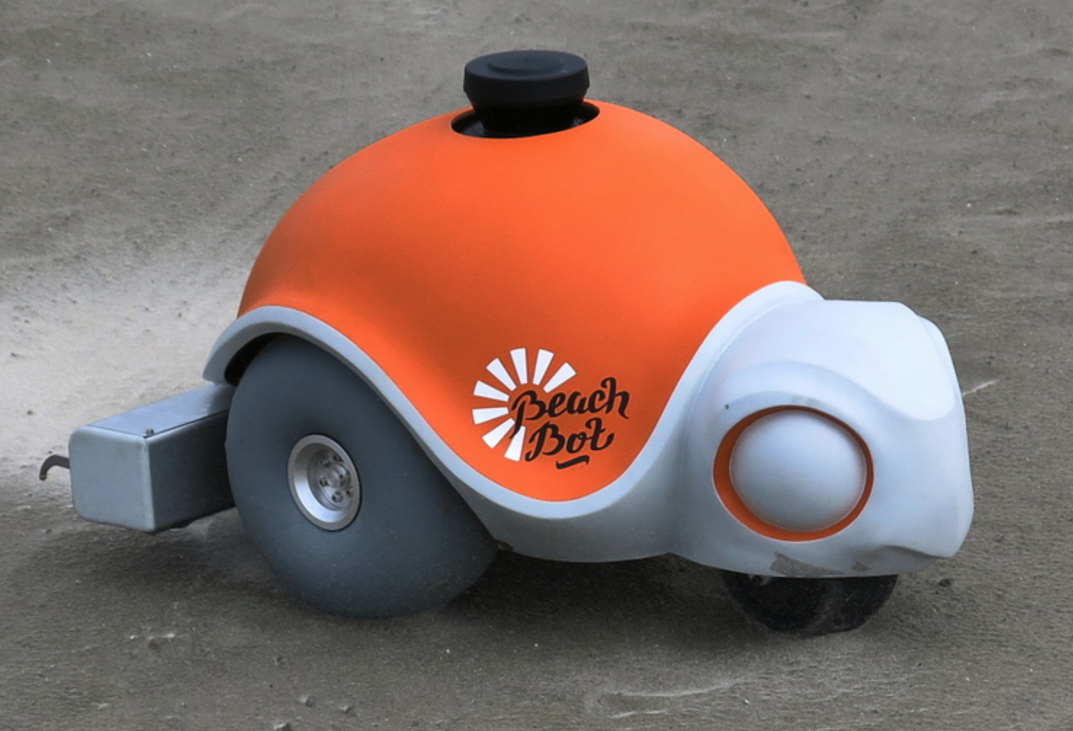
\includegraphics[width=0.43\textwidth]{Files/beachbot}
          \end{center}
          \caption{ETH Z\:urich's BeachBot robot.{\small (Retrieved from \citen{beachbot} on 2016--01--28)}}
          \label{fig: beachbot}
        \end{wrapfigure}
        The `best-in-class', and indeed only notable, beach-scale drawing robot is Disney's BeachBot (Figure~\ref{fig: beachbot}), produced by ETH Zurich.\cite{beachbot} The robot is capable of drawing images in the sand -- this has particular application in marketing Disney's sea themed--franchises and providing entertainment at Disney's beach resorts.\\
        The robot's drawing mechanism consists of fourteen rake teeth mounted in pairs on seven servo motors -- this allows lines of varying width (or no lines) to be drawn. The BeachBot is driven by two rear wheels and steered by a front wheel -- in a three-wheel configuration. It is fairly compact, measuring only sixty centimeters in length. BeachBot's chassis is enclosed in a sealed aluminum shell to protect its components from the sand. From this shell a laser scanner (part of BeachBot's guidance system) protrudes. The laser scanning guidance system directs BeachBot to draw its programmed image relative to reflecting posts installed by the user; this provides a `canvas' on which BeachBot works.\\
        BeachBot's shell is design to give it the appearance of a  turtle from Disney's \emph{Finding Nemo} property -- not only does this incorporate Disney's brand image into the design, but it also provides a non-threatening look. The latter point will be important for our robot since it will need to operate on a beach, an environment in which people are not used to seeing machinery.\\
        It has been suggested that with modification BeachBot could be used on snowy terrain to promote Disney's winter themed--franchises.

        \begin{wrapfigure}{O}{0.45\textwidth}
          \begin{center}
            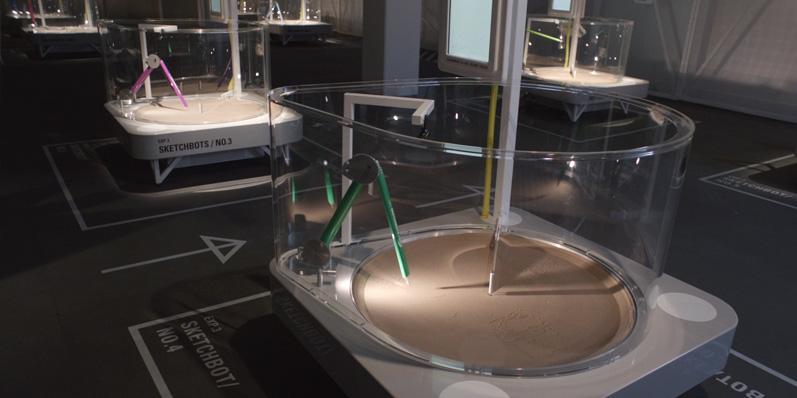
\includegraphics[width=0.43\textwidth]{Files/sketchbots}
          \end{center}
          \caption{Google Chrome Web Lab's sketchbots at the Science Museum, London.{\small (Retrieved from \citen{chromeweblab} on 2016--02--02)}}
          \label{fig: sketchbots}
        \end{wrapfigure}
        Although not beach-scale, Google has produced tabletop-scale sand art machines called `sketchbots' (Figure~\ref{fig: sketchbots}) (Operational at the Science Museum in London between 2012 and 2013).\cite{Warman2012} The robot itself was integrated with the tabletop; it comprised an arm with a mounted stylus and a `sweeping' implement, which moved in a circular motion, to clean the sand canvas. The robot took an input of the user's face from a camera, parsed the image and then drew it in the sand. Google  created the installation as part of its `Chrome Web Lab', showcasing modern web technologies such as HTML5.

\mySection{Robotics in education}{\SSB}\label{education review}
    The programming language Scratch was first released in 2005. It was designed by the Lifelong Kindergarten Group at the MIT Media Lab as a tool to introduce algorithmic thinking to 8--16 year-olds.\cite{scratch} The group state on their website that
    \begin{quotation}
        ``Scratch helps young people learn to think creatively, reason systematically, and work collaboratively -- essential skills for life in the 21st century.''
    \end{quotation}
    The inclusion of computational thinking in the primary science curriculum is gaining popularity. The ability to express the steps required to solve a given problem are important learning goals for children in a world where many rely on technology in the home, at work and in school.

    Furthermore, tools which allow students to employ these skills in the real world have proved to be very popular. The first programmable Lego product was released in 1989; since then the concept has been developed by numerous groups. Now there are several robotics platforms for educational purposes. The Lego group have several such platforms: the Lego Mindstorms range includes commercial packages as well as packages designed for schools. These allow high-school students to build embedded systems using different sensors and effectors to interact which can be programmed. The Mindstorms range forms the basis for the First Lego League competitions, which operate all over the world. MIT's Zero Robotics competitions also allow high- and middle-school students to program spherical robots on the International Space Station to solve challenges as part of an annual competition.\cite{zerorobotics}\\
    More recently, systems have been developed for younger students. Lego WeDo and WeDo 2.0 are designed for children aged 7--10 years to build simple robots and program them to perform actions using a software package based on Scratch.\cite{wedo2} This approach to robotics and programming has been designed in accordance with the US National Research Council's `Next Generation Science Standards'.

    \begin{wrapfigure}{I}{0.45\textwidth}
      \begin{center}
        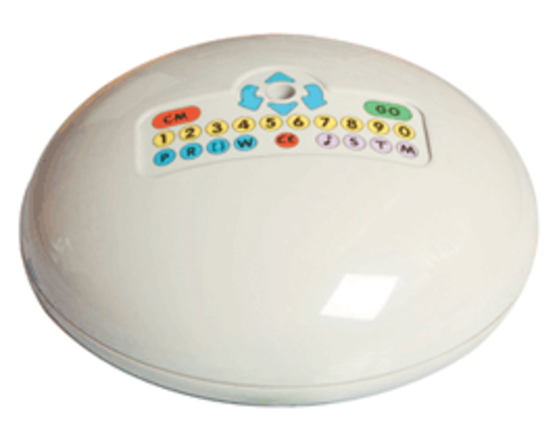
\includegraphics[width=0.43\textwidth]{Files/valiant_roamer.pdf}
      \end{center}
      \caption{The Valiant Technology Classic Roamer, a robot designed to teach algorithmic thinking to primary-age children. It is based on the Logo programming language. \small (Retrieved from \citen{valiantroamer} on 2015--01--18)}
      \label{fig: valiant roamer}
    \end{wrapfigure}
    However, none of the these technologies are new ideas: the programming language Logo was developed in 1967 as an educational tool. Among other features, Logo employed the idea of body-syntonic reasoning: processes are carried out relative to the current state, rather than relative to some reference state. One of Logo's creators, Seymour Papert, also invented a turtle robot (inspired by the tortoise robots developed by neurophysiologist William Grey Walter in the 1940s); this robot was programmed using Logo to move around a surface and draw patterns. It carried a pen and could be instructed to turn, move forwards and deploy or retract the pen. Using these simple commands, the turtle robot could be programmed to draw pictures and patterns on the surface over which it moved.\\
    Seymour Papert's turtles continue to be popular in primary schools across the world; the modern iteration is Valiant Technology's Roamer (Figure~\ref{fig: valiant roamer}).\cite{valiantroamer} Simple interfaces have been designed for the Roamer so it can be used without a programming language. Different models are available with different levels of complexity for different age ranges.

    \chapter{Preliminary Research}\label{research}\label{section \thechapter}

\mySection{Sand-drawing robots}{\SW}\label{sand-drawing robots}
    \begin{wrapfigure}{I}{0.45\textwidth}
      \begin{center}
        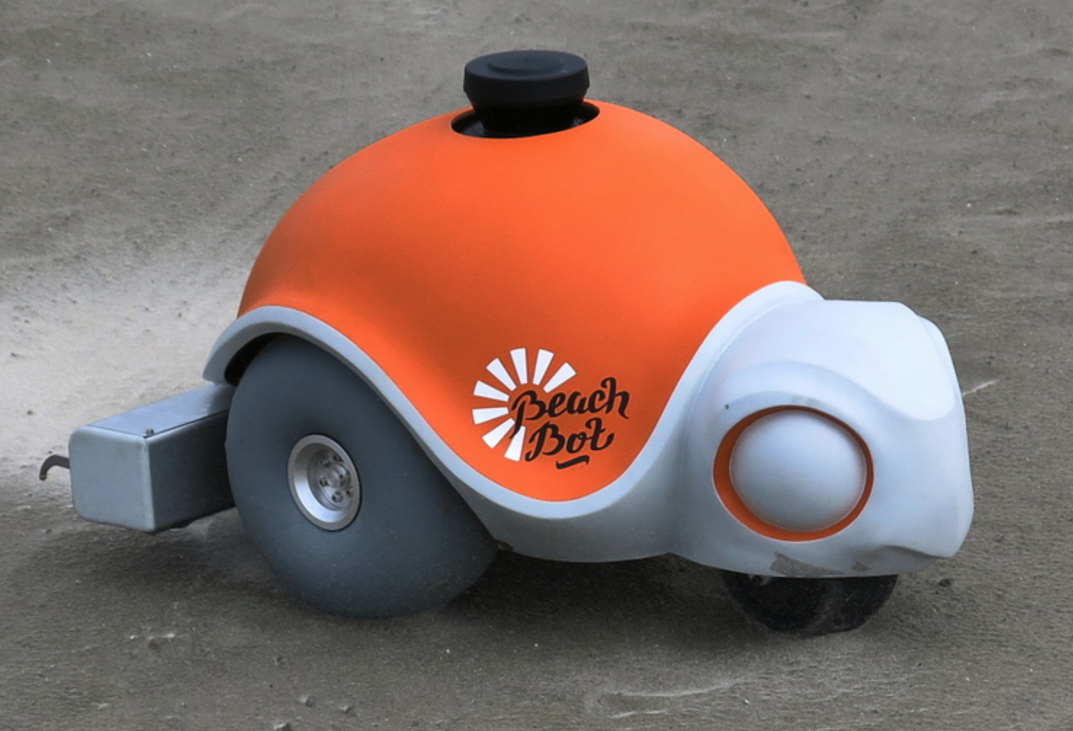
\includegraphics[width=0.43\textwidth]{Files/beachbot}
      \end{center}
      \caption{ETH Z{\"u}rich's BeachBot robot.{\small (Retrieved from \citen{beachbot} on 2016--01--28)}}
      \label{fig: beachbot}
    \end{wrapfigure}
    The `best-in-class', and indeed only notable, beach-scale drawing robot is Disney's BeachBot (Figure~\ref{fig: beachbot}), produced by ETH Z{\"u}rich.\cite{beachbot} The robot is capable of drawing images in the sand -- this has particular application in marketing Disney's sea themed--franchises and providing entertainment at Disney's beach resorts.\\
    The robot's drawing mechanism consists of fourteen rake teeth mounted in pairs on seven servo motors -- this allows lines of varying width (or no lines) to be drawn. The BeachBot is driven by two rear wheels and steered by a front wheel -- in a three-wheel configuration. It is fairly compact, measuring only sixty centimeters in length. BeachBot's chassis is enclosed in a sealed aluminum shell to protect its components from the sand. From this shell a laser scanner (part of BeachBot's guidance system) protrudes. The laser scanning guidance system directs BeachBot to draw its programmed image relative to reflecting posts installed by the user; this provides a `canvas' on which BeachBot works.\\
    BeachBot's shell is design to give it the appearance of a  turtle from Disney's \emph{Finding Nemo} property -- not only does this incorporate Disney's brand image into the design, but it also provides a non-threatening look. The latter point will be important for our robot since it will need to operate on a beach, an environment in which people are not used to seeing machinery.\\
    It has been suggested that with modification BeachBot could be used on snowy terrain to promote Disney's winter themed--franchises.

    \begin{wrapfigure}{O}{0.45\textwidth}
      \begin{center}
        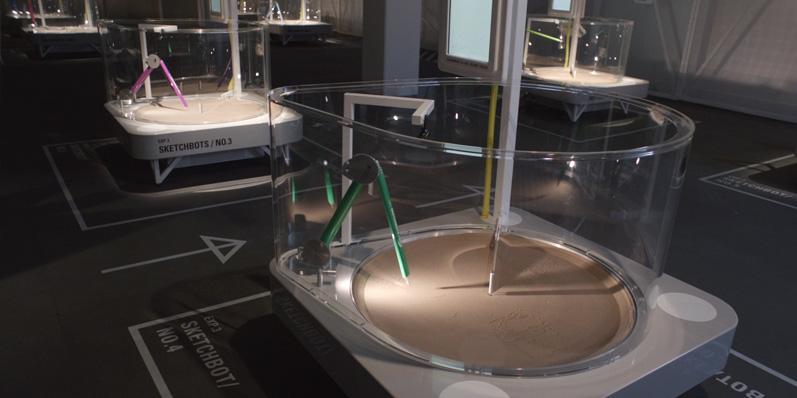
\includegraphics[width=0.43\textwidth]{Files/sketchbots}
      \end{center}
      \caption{Google Chrome Web Lab's sketchbots at the Science Museum, London.{\small (Retrieved from \citen{chromeweblab} on 2016--02--02)}}
      \label{fig: sketchbots}
    \end{wrapfigure}
    Although not beach-scale, Google has produced tabletop-scale sand art machines called `sketchbots' (Figure~\ref{fig: sketchbots}) (Operational at the Science Museum in London between 2012 and 2013).\cite{Warman2012} The robot itself was integrated with the tabletop; it comprised an arm with a mounted stylus and a `sweeping' implement, which moved in a circular motion, to clean the sand canvas. The robot took an input of the user's face from a camera, parsed the image and then drew it in the sand. Google  created the installation as part of its `Chrome Web Lab', showcasing modern web technologies such as HTML5.

\mySection{Movement}{\SW}
    In considering a robot's locomotion, the terrain over which it will travel (sand -- potentially damp) and its purpose (drawing) are center-stage. The robot must have sufficient traction to travel over a beach. When considering the requirement that it draw, it must be able to turn as tightly as instructed to avoid incongruity between programmed and drawn images. It may also be possible to incorporate any turning limitations into the child's programming interface, such that an impossible turn cannot be instructed. It would also be far from ideal for the robot to obscure any lines it had already drawn when pathing back over them.

    The main methods of robot locomotion that might be relevant are wheeled (or caterpillar tracked), walking, rolling, or slithering. Considering the scope of this project, and the budget available, the latter options are not viable. Companies such as Boston Dynamics have budgets of millions of dollars to work on the development of walking technology -- achieving a robot capable of walking is a significant feat, even before considering drawing. While rolling or slithering may potentially be workable, they would contribute significant design complications to any kind of `on/off' functionality. Flying private drones have increased in popularity dramatically; in considering a drone type robot as an option, the main challenges are the extreme comparative difficulty of achieving flight compared with traction and drawing a line in the sand. Creating a flying drone from scratch would pose many challenges, which it is unlikely we could surmount with this project's resources. The marker design also poses significant challenges -- a marker fixed rigidly to a drone is likely to interfere with flight and a free-hanging marker runs the risk of not providing enough pressure to create a line. The most viable locomotion solutions are caterpillar tracks and wheels.\\
    Caterpillar tracks combine very capable terrain handling with on-a-point turning, however they are very likely to disrupt the line left behind the robot, especially when on-a-point turning.  With the right design and material, wheels might prove sufficiently able to handle the terrain and also cause limited harm to the robot's drawn lines. Such wheels would need to have a large surface area and be made of a reasonably soft material (\eg soft touch plastic) -- minimizing the robot's overall weight would also be important in making such a design choice viable. Although wheels open opportunities in terrain handling and line preservation, they come up short of caterpillar tracks on turning ability. A short wheelbase might go some way to improve this. There is also the potential of a three-wheel configuration, instead of four (or more) wheels -- this was implemented in Disney's BeachBot (Section~\ref{sand-drawing robots}) to the benefit of the robot’s turning circle. It should be noted that a three-wheel design raises stability concerns. Ultimately the decision between caterpillar tracks and wheels comes to a question of whether, or to what extent, the child instructing the robot should be limited in their design.

\mySection{Digging mechanisms}{\SW}
    At its most basic level, a beach-scale sand drawing robot need only leave a line in the sand wherever it travels, in order to produce a picture -- this poses a severe constraint on what can be drawn. In the case of our educational robot, the child would have the limitation of instructing the robot to draw a picture with only a single continuous movement. This `always on' approach to the drawing mechanism can be improved upon.

    Instead of fixing the robot's marking implement, it could be built to raise or lower, adding `on/off' drawing functionality. The marking implement, or `marker', could be fitted to an actuator to achieve this. The actuator could be linear or rotary; a linear actuator would lend itself to a marker below the robot chassis, while a rotary actuator would be more appropriate for a marker behind the chassis, like a rake tooth (as is being used in Figure~\ref{fig: andres amador}). A rear mounted, rake-like design might provide a more fluid, pulling movement through the sand. There are precedents for this positioning choice: Disney's BeachBot (Section~\ref{sand-drawing robots}) and plough attachments for tractors. While the addition of an actuator significantly improves the robot's drawing flexibility, it would be vulnerable to sand in its mechanism and would add cost, should one not be salvageable from spare parts. The use of an actuator would also place a small requirement on the robot's power supply.\\
    The marker itself needs to exert sufficient force on the sand to leave a line behind the robot, without acting as a brake -- this would inhibit the robot's movement. Inhibition of the robot's movement would lead to significant deviation in the drawn image compared to the programmed image. The key to avoiding this is to create a marker with appropriate depth; the marker should not penetrate so deep in the sand as to invite significant resistance to its motion, while reaching deep enough to leave a sufficient (\emph{i.e.} visible) line.\\
    Implementing software to vary the depth of the marker could serve to mitigate any issues arising from resistance, and also could ensure trouble does not arise on uneven beach area. The limitations here lie within the realm of software development, and potentially the requirement that the actuator provide feedback.\\
    Within these parameters the marker itself could be varied -- for instance having multiple markers would provide a different pattern to the line. These multiple markers could be fitted to more actuators (with the potential of substantially increased cost) to allow for a variable line width.

    An alternative marker approach would be that of a cylindrical `drum'. Such a cylinder could have a pattern embossed upon it that would leave a pattern as the robot's marking. Gunilla Klingberg's `sand machine' (Section~\ref{art review}, Figure~\ref{fig: sand machine}) uses this approach. This approach could be implemented with `on/off' functionality, but would allow for only a preset pattern in the line. The implementation of a patterned line of varying width (\eg multiple drums with raising and lowering ability) could prove very problematic. Such an implementation of this method would be best achieved in a manner similar to NASA's RASSOR digging robot -- a drum separate from the locomotion mechanism that can be lowered and raised.\cite{Siceloff2013} In a similar way, the NASA's Curiosity rover leaves the pattern for ``JPL'' in Morse code in its tracks as it travels across the Martian surface.

\mySection{Construction materials}{\AK}
    An important consideration when deciding on a material for the body and base of the robot is the penetration into the sand. A denser material will cause the robot to sink more, but lighter materials will mean a compromise in strength, stability, or price. However, if the wheels or tracks of the robot are wise enough, there may be some freedom when deciding what materials the components of the robot should be made of.\\
    Researchers at the Georgia Institute of Technology have been able to vary the strength of the supporting ground by using varying air flow from beneath.\cite{Qian} This has allowed them to vary the stiffness of the sand and observe the performance of a robot on these surfaces.

    The robot should be made to be water resistant; contact with water at some point is inevitable and water coming into contact with the electrics would reduce the lifespan and reliability of the machine. Damage caused by sand should also be a consideration: the machine is likely to come into contact with a substantial amount of sand. Sand is silica, which is very abrasive; if this abrasion occurs around the more sensitive areas of the machine it could cause extensive damage. Sandusa is a range of beach products that are water- and sand-proof.\cite{sandusa} This is due to a smooth nylon material that allows sand to slide off easily combined with an inner waterproof lining. This material could be used to protect the robot.

    % In this section:
% This should contain all of the decisions regarding the design. If the reader has a question (`why did they do/choose that?' then this is where they look)

% Things to include here:
% Choosing motors
% Choosing gears/etc
% Choosing servos

\chapter{Design Outline}\label{design outline}\label{section \thechapter}\todo{Is this the best name for this chapter?}

\mySection{Aims and motivations}{\AH}\label{outline: aims and motivations}
    \towrite{aims and motivations}


\section{Robot body and movement}\label{outline: body and movement}

    \mySubsection{Chassis and materials}{\AK}
        An important consideration when deciding on a material for the body and base of the robot is the penetration into the sand. A denser material will cause the robot to sink more, but lighter materials will mean a compromise in strength, stability, or price. However, if the wheels or tracks of the robot are wise enough, there may be some freedom when deciding what materials the components of the robot should be made of.\\
        Researchers at the Georgia Institute of Technology have been able to vary the strength of the supporting ground by using varying air flow from beneath.\cite{Qian} This has allowed them to vary the stiffness of the sand and observe the performance of a robot on these surfaces.

        The robot should be made to be water resistant; contact with water at some point is inevitable and water coming into contact with the electrics would reduce the lifespan and reliability of the machine. Damage caused by sand should also be a consideration: the machine is likely to come into contact with a substantial amount of sand. Sand is silica, which is very abrasive; if this abrasion occurs around the more sensitive areas of the machine it could cause extensive damage. Sandusa is a range of beach products that are water- and sand-proof.\cite{sandusa} This is due to a smooth nylon material that allows sand to slide off easily combined with an inner waterproof lining. This material could be used to protect the robot.
        \towrite{materials and chassis}


    \mySubsection{Movement}{\SW}
        In considering a robot's locomotion, the terrain over which it will travel (sand -- potentially damp) and its purpose (drawing) are center-stage. The robot must have sufficient traction to travel over a beach. When considering the requirement that it draw, it must be able to turn as tightly as instructed to avoid incongruity between programmed and drawn images. It may also be possible to incorporate any turning limitations into the child's programming interface, such that an impossible turn cannot be instructed. It would also be far from ideal for the robot to obscure any lines it had already drawn when pathing back over them.

        The main methods of robot locomotion that might be relevant are wheeled (or caterpillar tracked), walking, rolling, or slithering. Considering the scope of this project, and the budget available, the latter options are not viable. Companies such as Boston Dynamics have budgets of millions of dollars to work on the development of walking technology -- achieving a robot capable of walking is a significant feat, even before considering drawing. While rolling or slithering may potentially be workable, they would contribute significant design complications to any kind of `on/off' functionality. Flying private drones have increased in popularity dramatically; in considering a drone type robot as an option, the main challenges are the extreme comparative difficulty of achieving flight compared with traction and drawing a line in the sand. Creating a flying drone from scratch would pose many challenges, which it is unlikely we could surmount with this project's resources. The marker design also poses significant challenges -- a marker fixed rigidly to a drone is likely to interfere with flight and a free-hanging marker runs the risk of not providing enough pressure to create a line. The most viable locomotion solutions are caterpillar tracks and wheels.\\
        Caterpillar tracks combine very capable terrain handling with on-a-point turning, however they are very likely to disrupt the line left behind the robot, especially when on-a-point turning.  With the right design and material, wheels might prove sufficiently able to handle the terrain and also cause limited harm to the robot's drawn lines. Such wheels would need to have a large surface area and be made of a reasonably soft material (\eg soft touch plastic) -- minimizing the robot's overall weight would also be important in making such a design choice viable. Although wheels open opportunities in terrain handling and line preservation, they come up short of caterpillar tracks on turning ability. A short wheelbase might go some way to improve this. There is also the potential of a three-wheel configuration, instead of four (or more) wheels -- this was implemented in Disney's BeachBot (Section~\ref{sand-drawing robots}) to the benefit of the robot’s turning circle. It should be noted that a three-wheel design raises stability concerns. Ultimately the decision between caterpillar tracks and wheels comes to a question of whether, or to what extent, the child instructing the robot should be limited in their design.
        \towrite{movement: the decision}


    \mySubsection{Digging mechanisms}{\SW}\label{outline: drawing tool}
        At its most basic level, a beach-scale sand drawing robot need only leave a line in the sand wherever it travels, in order to produce a picture -- this poses a severe constraint on what can be drawn. In the case of our educational robot, the child would have the limitation of instructing the robot to draw a picture with only a single continuous movement. This `always on' approach to the drawing mechanism can be improved upon.

        Instead of fixing the robot's marking implement, it could be built to raise or lower, adding `on/off' drawing functionality. The marking implement, or `marker', could be fitted to an actuator to achieve this. The actuator could be linear or rotary; a linear actuator would lend itself to a marker below the robot chassis, while a rotary actuator would be more appropriate for a marker behind the chassis, like a rake tooth (as is being used in Figure~\ref{fig: andres amador}). A rear mounted, rake-like design might provide a more fluid, pulling movement through the sand. There are precedents for this positioning choice: Disney's BeachBot (Section~\ref{sand-drawing robots}) and plough attachments for tractors. While the addition of an actuator significantly improves the robot's drawing flexibility, it would be vulnerable to sand in its mechanism and would add cost, should one not be salvageable from spare parts. The use of an actuator would also place a small requirement on the robot's power supply.\\
        The marker itself needs to exert sufficient force on the sand to leave a line behind the robot, without acting as a brake -- this would inhibit the robot's movement. Inhibition of the robot's movement would lead to significant deviation in the drawn image compared to the programmed image. The key to avoiding this is to create a marker with appropriate depth; the marker should not penetrate so deep in the sand as to invite significant resistance to its motion, while reaching deep enough to leave a sufficient (\emph{i.e.} visible) line.\\
        Implementing software to vary the depth of the marker could serve to mitigate any issues arising from resistance, and also could ensure trouble does not arise on uneven beach area. The limitations here lie within the realm of software development, and potentially the requirement that the actuator provide feedback.\\
        Within these parameters the marker itself could be varied -- for instance having multiple markers would provide a different pattern to the line. These multiple markers could be fitted to more actuators (with the potential of substantially increased cost) to allow for a variable line width.

        An alternative marker approach would be that of a cylindrical `drum'. Such a cylinder could have a pattern embossed upon it that would leave a pattern as the robot's marking. Gunilla Klingberg's `sand machine' (Section~\ref{art review}, Figure~\ref{fig: sand machine}) uses this approach. This approach could be implemented with `on/off' functionality, but would allow for only a preset pattern in the line. The implementation of a patterned line of varying width (\eg multiple drums with raising and lowering ability) could prove very problematic. Such an implementation of this method would be best achieved in a manner similar to NASA's RASSOR digging robot -- a drum separate from the locomotion mechanism that can be lowered and raised.\cite{Siceloff2013} In a similar way, the NASA's Curiosity rover leaves the pattern for ``JPL'' in Morse code in its tracks as it travels across the Martian surface.

\section{Electronics and control}\label{outline: electronics and control}
    \mySubsection{Guidance methods}{\CL \SW}\label{outline: guidance}
        In order to draw an image in a given area, the robot will need to be guided by some system. \towrite{Guidance: manual controls}

        The robot could also be autonomous. Three options for autonomous guidance have been explored: ultrasound, lasers, and \gls{GPS}. There are many other guidance systems that have not been mentioned such as tethering, grid systems, infrared, and more. These other guidance systems have not been mentioned because they are either too complex, have too small of a range, or it is not possible to make an autonomous robot using the particular guidance system.

        \paragraph{Ultrasound} detection systems comprise two parts, a transmitter and a receiver. The transmitter emits a sound at a defined frequency (typically around \SI{40}{\kilo\hertz}) and the receiver collects the sound reflected back by the obstacles. The distance to the objects is calculated by measuring the time taken by the sound to return to the receiver.\\
        Ultrasound is normally used to measure distances because sensors because they are cheap and very simple to use. Ultrasound has a range of \SIrange{1}{250}{\centi\meter} and an effective working angle of approximately 30\dg.\cite{ultrasoundrobots} The working angle of ultrasound can be pictured as a cone that has an angle of 30\dg, where measurements of distance will be more accurate within the centre of the cone and less accurate towards the sides. Other things to be considered with ultrasound are the shape of the obstacle and the inability of ultrasound to make measurements of distance when the sensor is very close to an obstacle. This is due to the sensor needing a large enough return time for the wave that is reflected; if the a sensor with a long transmitting wave duration is used, it may not be able to detect an object in close proximity since the wave will return too quickly, before the sensor can started receiving.\\
        Ultrasound is normally used to measure distances because sensors because they are cheap and very simple to use. Ultrasound has a range of \SIrange{1}{250}{\centi\meter} and an effective working angle of approximately 30\dg.\cite{ultrasoundrobots} The working angle of ultrasound can be pictured as a cone that has an angle of 30\dg, where measurements of distance will be more accurate within the centre of the cone and less accurate towards the sides. Other things to be considered with ultrasound are the shape of the obstacle and the inability of ultrasound to make measurements of distance when the sensor is very close to an obstacle. This is due to the sensor needing a large enough return time for the wave that is reflected.\todo{how would US be used to guide the robot to draw an image?}

        \paragraph{Lasers} could be used in different ways to guide the robot. One way is to have a guidance system for freely chosen courses, which uses a laser beam that hits strategically placed mirrors to reflect the beam. The on-board controller then analyses the angles that the beam is reflected at and uses triangulation to determine the position of the robot. Another method is to use a laser range finder that emits a beam and measures the time taken to reflect off the object and return to the sender. Both methods are accurate to within a few millimetres but the first method is the more accurate of the two.\\
        Laser guidance systems can be used in any environment and have a range of several metres. They have a range of several metres and out of the three guidance systems mentioned are the most accurate. The markers for the laser beams have to be set every \SIrange{2.5}{4.5}{\meter} and should not be blocked. The robot must be able to see multiple markers (mirrors) at once so that it can determine its precise location. The only disadvantages of using a laser guidance system are that they are the most complicated and the most expensive of the three systems discussed.\todo{mention LIDAR?}

        \paragraph{\gls{GPS}} receivers use a constellation of 31 satellites orbiting over 20,000 km, with a revolution period of 12 hours (as of February 1st 2016). Every satellite transmits data packs, which contains: the time, current position, other satellites positions and other information. The \gls{GPS} receiver receives the information about position from the radio transmissions of the satellites it can track. 4 satellites are normally used to compute the position. Although it is possible to measure the position with fewer satellites, the margin of error is large.\\
        \gls{GPS} \glspl{shield} are inexpensive and as a guidance system, obviously have a very large range.  However, the accuracy of \gls{GPS}, which may be within few metres, may depend a number of things such as signal noise, satellite position, and obstruction from tall buildings. Therefore, if GPS is to be used as the guidance system for the robot, then its worth considering a location that is isolated from tall building when it comes to the testing of the robot because signal noise can cause errors up to \SI{10}{\meter} and obstruction from tall buildings can cause errors three times more than the error from signal noise.\cite{gpsbasics} There are ways of getting the accuracy of the \gls{GPS} down to a few centimetres by using correction methods such as a differential \gls{GPS}, using a combination of \gls{GPS} and some other local positioning systems such as electronic compasses or \gls{INS}. However, these correction methods are complex and expensive and therefore they are not feasible solutions to increasing the accuracy of \gls{GPS}.

        \towrite{electronics: kill switch}


    \mySubsection{Control platform}{\SSB}\label{outline: control}
        \begin{figure}%{I}{0.45\textwidth}
            % \vspace{-11pt}
            \centering
            \begin{subfigure}[b]{0.45\textwidth}
                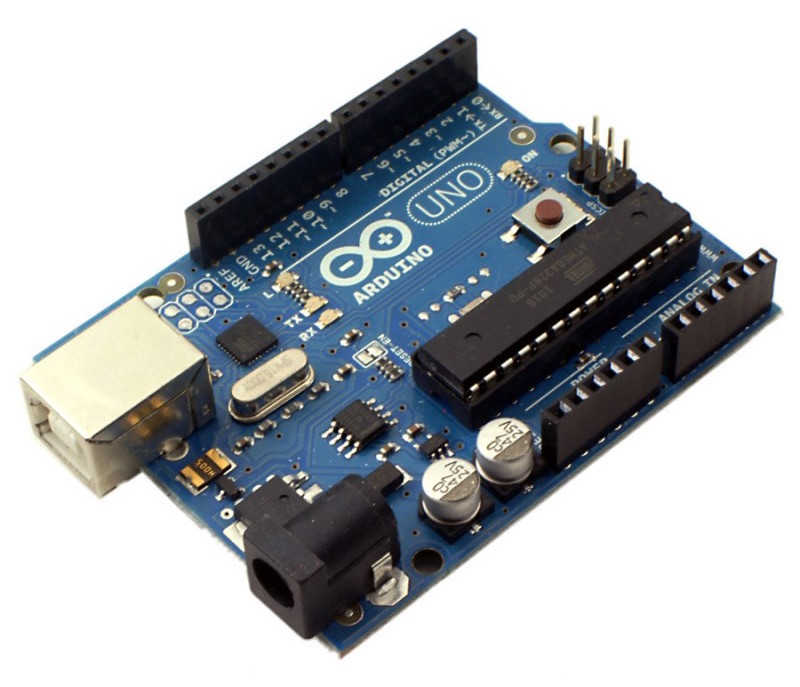
\includegraphics[width=\textwidth]{Files/arduino}
                \caption{An Arduino UNO.}
                \label{fig: arduino}
            \end{subfigure}
            ~
            \begin{subfigure}[b]{0.45\textwidth}
                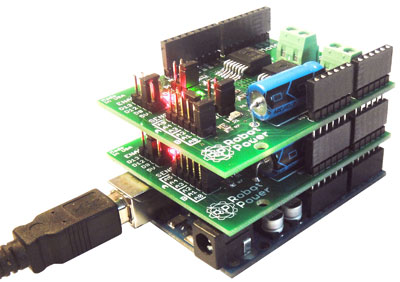
\includegraphics[width=\textwidth]{Files/arduino_with_shields}
                \caption{An Arduino with 2 \glspl{shield} attached.}
                \label{fig: arduino shields}
            \end{subfigure}
            \caption{\small (Retrieved from \citen{robotshop} on 2016--01--25)}
            \label{fig: arduino and shields}
            % \vspace{-20pt}
        \end{figure}
        The robot will need a control system to plan and control its movement, and to control the drawing tool. This system could be developed from proprietary systems or built by the group for this specific application.

        \paragraph{\gls{Arduino}} (Figure~\ref{fig: arduino}) is an open-source micro-controller system designed for embedded systems control. It can be expanded by the use of \emph{\glspl{shield}} (Figure~\ref{fig: arduino shields}), circuit boards designed to attach to header pins on the primary micro-controller board to created stacks of circuits with different functions. This would allow us to build a control system for the robot using pre-designed circuits. \Glspl{shield}, which can be bought from many electronics suppliers, are available to add bluetooth, GPS, motor control, and many other functions to the primary circuit.\\
        There is a large online community supporting the \gls{Arduino} project, which could be leveraged to solve programming difficulties if they arise. The \gls{Arduino} project provides an integrated development environment (IDE); the \gls{Arduino} is programmed using a language based on the C and C++ languages.
        \paragraph{Netduino} is a variant of the \gls{Arduino} which runs on Microsoft's .NET framework. The online support community for this system is smaller, although some group members (\AG, \LY) have a pre-existing familiarity with the .NET framework.\\

        \todo[inline]{electronics: rework the following paragraphs}
        \paragraph{Raspberry Pi} is a small single-board computer developed in the UK to promote access to computer science education in schools. Because on this, the platform is already widely used in an educational setting and thus would allow this project to be more easily integrated into the teaching of computer science. The computer itself is low-cost (<\pounds{50}\todo{check the price of Raspberry Pi}).\\
        The Raspberry Pi Foundation also produce smaller versions of the Raspberry Pi computer which are designed for use in embedded systems. These boards are less customizable than the Arduino system. However, it is compatible with the Python language, which has an extensive support community online and is familiar to all the group, as well as C, C++, Java, and others.

        \paragraph{A micro-controller} integrated circuit could be used in a purpose-built system to control the robot. This would require the design of all the supporting electronics. The microprocessor would need to be programmed in a low-level assembly language or a language designed specifically for the micro-controller product we use.\\
        These components would be cheaper than commercially available systems, but would require much more electronics design work and fabrication.

        \mySubsection{Power}{\SSB}\label{outline: power}
            The \gls{Arduino} requires a supply voltage of \SIrange{7}{12}{\volt}. The motors will also require a power supply of \SIrange{5}{12}{\volt}. There are many different types of battery, several of which are appropriate for the robot:

            \paragraph{Single-use alkaline} batteries are common-place and cheap. They come in a variety of sizes and capacities. These batteries must be disposed of after use and can only source small currents (typically no more than 1A). \SI{9}{\volt} PP3 batteries are particularly popular for electronics projects due to their regular shape and convenient connections.
            \paragraph{Rechargeable alkaline or nickel-based} batteries can be re-used. They are often more efficient than their single-use counterparts.
            \paragraph{Lithium Polymer} batteries are often used for remote-controlled vehicles. They have a very high energy-density and can source high currents (>\SI{10}{\ampere}). This makes them particularly suited to powering small vehicles. These batteries are also rechargeable and have short charging times.

            \paragraph{}In order to allow the motors to sink high currents without affecting the supply voltage to the micro-controller, separate power supplies are used for each system: the \gls{Genuino}, the GPS shield and the \gls{magnetometer} (the control system); and the motors and \glspl{servo} (the output system). The lithium polymer batteries are the best choice for the motors since they can source the required currents and are light-weight. The capacity of the battery for the output system is a matter of cost; a high-capacity battery is more convenient but will be more expensive.\\
            The simplest power source for the control system is a \SI{9}{\volt} PP3 battery. The output system is driven by a \SI{7.4}{\volt} \SI{1500}{\milli\ampere\hour} lithium polymer battery\footnote{\pounds{12.00} from Component Shop \textsc{URL:} \url{www.componentshop.co.uk}~~~~\texttt{SKU: LN215}}. This can supply a continuous current of up to \SI{52.5}{\ampere} and can drive both motors at maximum power for 23 minutes. The control and output systems must have a common ground (\SI{0}{\volt}) connection.

    \mySubsection{Motors}{writer TBA}\label{outline: motors}
    \towrite{motors}

\mySection{User interface}{writer TBA}
    \towrite{interface}


\section{Summary and decisions}
    \towrite{summary and decisions}
    \myBlindSubsection{Aims and motivations}{\AH}
    It was agreed by the group that the aim of this project would be the produce a sand art--drawing robot for educational purposes. The intention being that the final product may be utilised to teach pupils, of primary school age, the basic steps involved in coding.
    The children would input a design, using preliminary coding language, into an interface. The children would have to consider the steps involved in producing their desired image and input the details in a manner that a computer can understand. The group's robot would then reproduce this design in the sand.




    \myBlindSubsection{Drawing tool}{writer TBA}


    \myBlindSubsection{Electronics platform and guidance system}{writer TBA}

    Separate power supplies are used for the control system and the motors. The power source for the control system is a \SI{9}{\volt} PP3 battery. The motors are driven by a \SI{7.4}{\volt} \SI{1500}{\milli\ampere\hour} lithium polymer battery.


    \mySubsection{Outline specification}{\textsc{Whole Group}}\label{outline specification}
        \begin{enumerate} %Reference items in this list using \refspec{drawing size} etc.
            \subsubsection{The project}
            \item We shall design and build a prototype robot to draw 2d line drawings in sand.\label{spec: draw}
            \item The robot shall take input from a user which it shall translate into instructions to draw the picture;\label{spec: take input}
            \item the drawings should be ??? \todo{how big will the drawings be?} in size; \label{spec: drawing size}
            \item the robot should be for educational uses. \label{spec: education}

            \subsubsection{Control systems}
            \item The robot shall be controlled with a \gls{Genuino} 101; \label{spec: arduino}
            \item the robot shall use \gls{GPS} for guidance; \label{spec: gps}
            \item the robot should detect objects in front of it. The robot should not collide with objects; \label{spec: detect objects}
            \item the robot should circumvent obstacles.\label{spec: circumvent}

            \subsubsection{The robot hardware}
            \item The robot shall move across the sand using ???\todo{how will it move?}; \label{spec: movement}
            \item the robot shall use ??? \todo{how will it draw?} to draw the images; \label{spec: tool}
            \item the robot shall be built from ??? \todo{what will it be built from?}; \label{spec: material}
            \item the robot shall have dimensions equal to or less than ($56 \times 45 \times 25$) cm. \label{spec: robot size}

            \subsubsection{Safety}
            \item The robot shall have an emergency shut-down switch; \label{spec: kill switch}
            \item the robot should indicate operating faults to the user; \label{spec: error indicator}
            \item the robot should have documentation and instructions for end users. \label{spec: documentation}
        \end{enumerate}

    % In this section:
% Someone should be able to build a robot just like ours from the information in this section.
% Include all drawings, specifications, decisions and processes.

\chapter{Design Specification}\label{design specification}\label{section \thechapter}

% Here: Description of what the robot should do/be

\mySection{Robot design and hardware}{writer TBA}
\towrite{hardware}


\mySection{Electronics and control systems}{writer TBA}
\towrite{electronics}


\mySection{Software and user interface}{writer TBA}
\towrite{software}


\mySection{Other considerations}{writer TBA}
\towrite{other considerations}

    % In this section:
% Plan the manufacture process step by step.

\chapter{Plan of Manufacture}\label{manufacture plan}\label{section \thechapter}
The first functioning prototype of the \SandE robot was built from the designs in section \ref{design specification} according to the following plan.

\begin{multicols}{2}
\begin{enumerate}

    \section{Chassis}

    \section{Electronics and control systems}
        \item buy box
        \item Cut holes in electronics housing
        \item Attach the grommets to the electronics housing
        \item Solder spade connectors to the motor cables
        \item Thread all cables through the appropriate holes in the housing and through the nut for the switch
        \item Solder the \SI{2.1}{mm} jack plug to cables
        \item Solder the positive jack plug cable to the switch
        \item Solder the \SI{0}{\volt} jack plug cable and the \SI{0}{\volt} connection of the tamiya connector to the c terminal of the \SI{9}{\volt} battery box
        \item Solder the positive connection of the tamiya connector to the switch
        \item Solder the \SI{9}{\volt} battery box to the switch
        \item Install the \SI{9}{\volt} battery box
        \item Install the switch
        \item Solder the headers to the \gls{servo} \gls{shield}
        \item Connect the \glspl{shield} together and to the \gls{Genuino}
        \item Solder the cables to the \gls{magnetometer} breakout board
        \item Connect the \gls{magnetometer} to the stack of Arduino \glspl{shield}
        \item Cut the VIN and \SI{5}{\volt} pins between the control section and the output section
        \item Screw the stack of Arduino \glspl{shield} and the \gls{magnetometer} to the housing base
        \item Feed the motor and \gls{servo} cables through grommets and attach them to the stack of Arduino \glspl{shield}
        \item Screw the strain relief sections onto the grommets

    \section{Integrating systems}
        \item Attach the base of the electronics housing to the chassis
        \item Attach all connectors to the electronics system
        \item Attach the electronics housing to its base

\end{enumerate}
\end{multicols}

    \chapter{Software}\label{software}\label{section \thechapter}

\begin{listing}[h!]
    \inputcode{6}{9}{test.ino}
    \caption{Example of some code in a listing. {\small (From \texttt{test.ino})}}%
    \label{lst: example}
\end{listing}



    % A final summary. This should form the basis of the Executive Summary, but this final summary gives you the opportunity to give more supporting detail for someone who wants more - but not a great deal more - information than in the Executive Summary.
% ---from the project guidance

\chapter{Summary}\label{summary,conclusion}\label{section \thechapter}
\glsresetall


\mySection{Background and objectives}{\AG}\label{summary: why}\label{summary: introduction}\todo{title of this section needs thought}
The invention of the difference engine in 1833, came with it an entire new process of thought and development. Since then, the field of computation and robotics has become one of the largest in the world. It is a field that requires developers to suspend their usual way of thinking and instead look at tasks and problems as a computer. These ways of thinking are not encountered in daily life. Other intellectual and physical fields have their foundations discovered through juvenile interactions. However, the ability to approach a task with an algorithmic method---a loop or conditional statements---is not naturally acquired. These skills must therefore be taught through non-conventional means. This could be as a teenager or adult, when first being confronted with programming; however, years of educational studies have shown that skills and understanding are much more easily acquired at an early age. This is the motivation of the \SandE project: to develop a method, useable by schools and parents, to begin to nurture programming skills in children.

The aim for the \SandE project is to develop a working prototype of a programmable, autonomous robot with the ability to draw large scale art in sand. The robot will be able to accept a set of repeatable instructions from a student. These instructions could include: navigation, for example an instruction to go from point A to B before turning and traveling to point C; the ability to control whether the robot should be drawing at any given time, and also the thickness of the line drawn. The student will create these instructions through a graphical user interface, before they are uploaded to the robot and their design is created in sand. The intention is that by passing a design to a robot, students will be forced to think about how a computer will tackle a task they would find simple. Hopefully, students will be able to understand that computers use a system of specific logic that can create wonderful things, which would take much longer by hand.



%Include the references
\cleardoublepage
\fancyhead[RO]{References}
\bibliographystyle{unsrtnat}
\bibliography{../library}
\cleardoublepage
\fancyhead[RO]{Glossary}
\printnoidxglossaries

%Begin annexes
\cleardoublepage
\fancyhead[RO]{\chaptertype~\thechapter: \small\nameref{section \thechapter}}
\appendix
\makeatletter
\renewcommand{\@chapapp}{Annex}
\makeatother
\renewcommand{\chaptertype}{Annex}
%Annexes of report
    \chapter{List of Components}\label{list of components}\label{section \thechapter}
\todo[inline]{Check appropriate page-breaks in this table}
% \centering
% \begin{longtable}{|l|}
%   ... your table ...
% \end{tabular}

\begin{longtable}{|c|p{0.2\textwidth}|p{0.15\textwidth}|p{0.12\textwidth}|}
% KILLED & LINE!!!! \kill
\hline\hline
% \multicolumn{5}{c}%
% {This part appears at the top of the table}\\
\textsc{Component}&\textsc{Manufacturer}&\textsc{Supplier}&\textsc{Stock \#}\\
\hline\hline
\endfirsthead
\caption[]{(continued)}\\
\hline\hline
% \multicolumn{5}{c}%
% {This part appears at the top of every other page}\\
\textsc{Component}&\textsc{Manufacturer}&\textsc{Supplier}&\textsc{Stock \#}\\
\hline\hline
\endhead
\hline\hline
% This goes at the&bottom.\\
\multicolumn{4}{|c|}%
{\emph{Continued overleaf}}\\
\hline\hline
\endfoot
\hline\hline
\multicolumn{4}{|c|}%
{\emph{End of list}}\\
\hline\hline
\endlastfoot
% \component{name}{model}{manufacturer}{supplier}{number}
    \multicolumn{4}{|c|}{\textsc%
    {Chassis and digging mechanism}}\\ \hline
        \component{Electronics housing}{Project Box 125$\times$80$\times$50mm}{Hammond}{Maplin}{N24HG}
    \hline\hline
    \multicolumn{4}{|c|}{\textsc%
    {Electronics and control}}\\ \hline
        \component{Arduino}{Genuino 101}{Arduino}{RS Components}{913--9999}
        \component{Motor shield}{Arduino Motor Shield Rev3}{Arduino}{RS Components}{758--9349}
        \component{GPS shield}{GPS Shield With SD Card Slot for Arduino}{LinkSprite}{Maplin}{N94DG}
        \component{Magnetometer}{Triple-axis Accelerometer + Magnetometer (Compass) Board}{Adafruit}{Maplin}{N46DQ}
        \component{Servo shield}{Motor/Stepper/Servo Shield for Arduino v2}{Adafruit}{Maplin}{A61QN}
    \hline\hline
    \multicolumn{4}{|c|}{\textsc%
    {Power}}\\ \hline
        \component{Battery}{7.4V 1500mAh 35C+ continuous discharge lipo battery}{Giant-Power}{Component Shop}{LN215}
    \hline\hline
    \multicolumn{4}{|c|}{\textsc%
    {Motors and movement}}\\ \hline
        \component{Motor}{919D Series 35mm single ratio (148:1) metal gearbox}{MFA ComoDrills}{}{RE-540/1}
        \component{Servo motors}{~}{~}{unknown}{N/A}
        \component{Cables}{Remote Control Servo Extension Cord Cable Wire}{unknown}{sourcingmap (Amazon)}{N/A}
    \hline\hline
    \multicolumn{4}{|c|}{\textsc%
    {Miscellaneous}}\\ \hline
        % \component{Battery box}{9V Switched Battery Box}{Maplin}{Maplin}{L90AN}
        \component{Battery box}{Panel Mount Battery Holder for 2, Solder Tag Contact}{Bulgin}{RS Components}{501--244}
        \component{Switch}{Miniature 6A AC 230V Rocker Switch DPDT}{Maplin}{Maplin}{YX65V}
        \component{Grommet}{Cable Exit Gland 15mm with Sleeve}{Maplin}{Maplin}{JZ43W}
        \component{Plug}{2.1 $\times$ 5.5mm DC Power Plug}{Maplin}{Maplin}{HH60Q}
        \component{Connectors}{Lucar Male}{Maplin}{Maplin}{JH90X}
        \component{Connectors}{Insulated Lucar Female}{Maplin}{Maplin}{JH82D}
        \component{Wire}{Equipment Wire 24-0.2mm}{Maplin}{Maplin}{BA40T KR31J BA42V}


\end{longtable}

    \chapter{Code for Genuino}\label{code}\label{section \thechapter}

% \lstinputlisting[caption={Test program for the motors}]{Code/test.ino}

\myBlindSubsection{test\_routine.ino}{\AG}\label{ino:test_routine}
This \gls{sketch} allows the robot's moving components to be tested.
\inputminted{cpp}{Code/test_routine.ino}

\myBlindSubsection{test\_routine.ino}{\AG}\label{ino:gps_navigation}
This \gls{sketch} \towrite{What does \texttt{gps\_navigation.ino} do?}.
\inputminted{cpp}{Code/gps_navigation.ino}

    \chapter{Board Meeting Minutes}\label{minutes}\label{section \thechapter}
\writers{Minutes kept and compiled by \SSB}

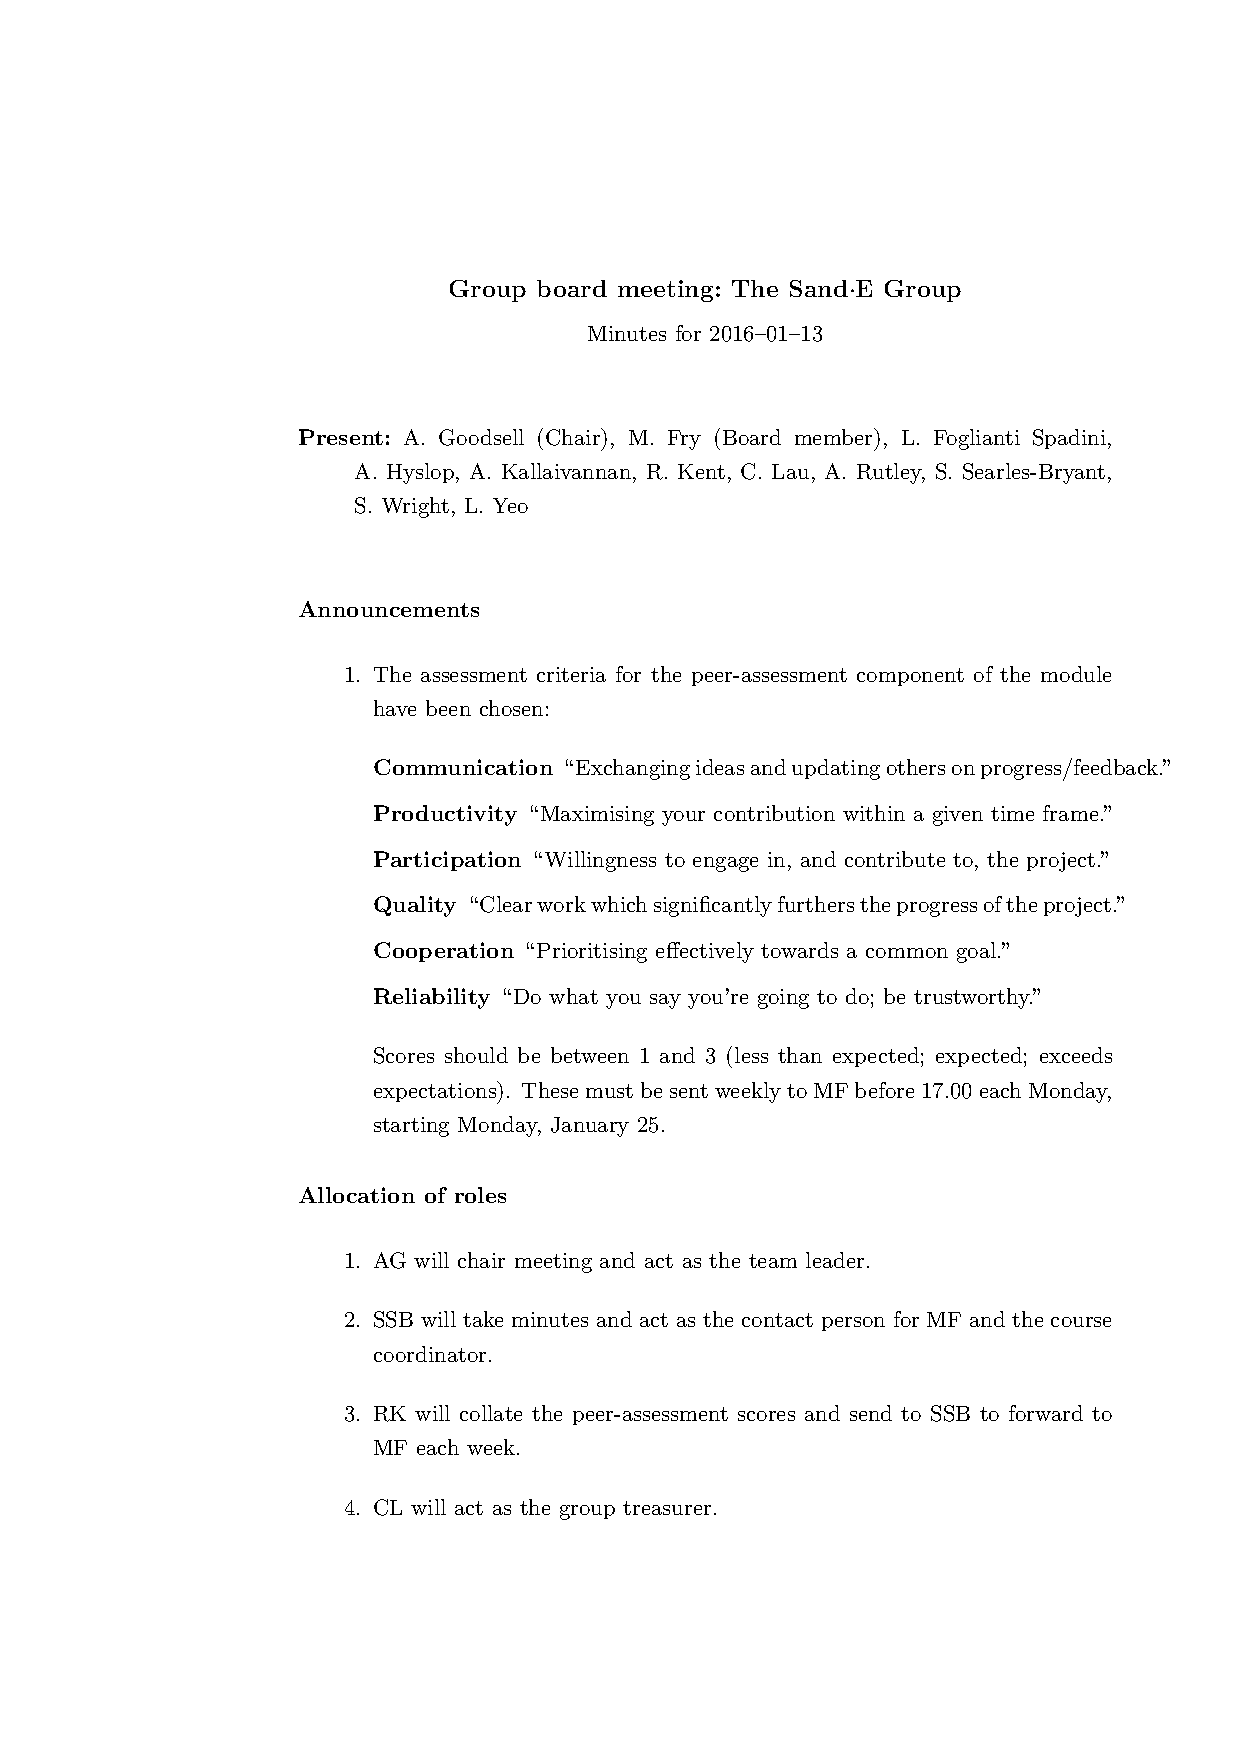
\includepdf[pages=-,pagecommand={\pagestyle{fancy}}]{Files/boardMeetingMinutes}

    \chapter{\teamname}\label{group}\label{section \thechapter}
\todo[inline]{Check you all approve of these photos. If not, please supply a 2:3 photo.}
\newpage
\captionsetup[subfigure]{labelformat=empty}

\begin{figure}
    % \vspace{-11pt}
    \centering
    \begin{subfigure}[b]{0.45\textwidth}
        \centering
        
\includegraphics[height=0.3\textheight]{Files/AG}
        \caption{Alexander Goodsell}
    \end{subfigure}
    ~~~~
    \begin{subfigure}[b]{0.45\textwidth}
        \centering
        
\includegraphics[height=0.3\textheight]{Files/LFS}
        \caption{Lorenzo Foglianti Spadini}
    \end{subfigure}\\
    \vspace{0.5cm}
    \begin{subfigure}[b]{0.45\textwidth}
        \centering
        
\includegraphics[height=0.3\textheight]{Files/AH}
        \caption{Ashleigh Hyslop}
    \end{subfigure}
    ~~~~
    \begin{subfigure}[b]{0.45\textwidth}
        \centering
        
\includegraphics[height=0.3\textheight]{Files/AK}
        \caption{Arunyan Kallaivannan}
    \end{subfigure}\\
    \vspace{0.5cm}
    \begin{subfigure}[b]{0.45\textwidth}
        \centering
        
\includegraphics[height=0.3\textheight]{Files/RK}
        \caption{Robert Kent}
    \end{subfigure}
    ~~~~
    \begin{subfigure}[b]{0.45\textwidth}
        \centering
        
\includegraphics[height=0.3\textheight]{Files/CL}
        \caption{Calvin Lau}
    \end{subfigure}
\end{figure}
\begin{figure}
    % \vspace{-11pt}
    \centering
    \begin{subfigure}[b]{0.45\textwidth}
        \centering
        
\includegraphics[height=0.3\textheight]{Files/AR}
        \caption{Alan Rutley}
    \end{subfigure}
    ~~~~
    \begin{subfigure}[b]{0.45\textwidth}
        \centering
        
\includegraphics[height=0.3\textheight]{Files/SSB}
        \caption{Samuel Searles-Bryant}
    \end{subfigure}\\
    \vspace{0.5cm}
    \begin{subfigure}[b]{0.45\textwidth}
        \centering
        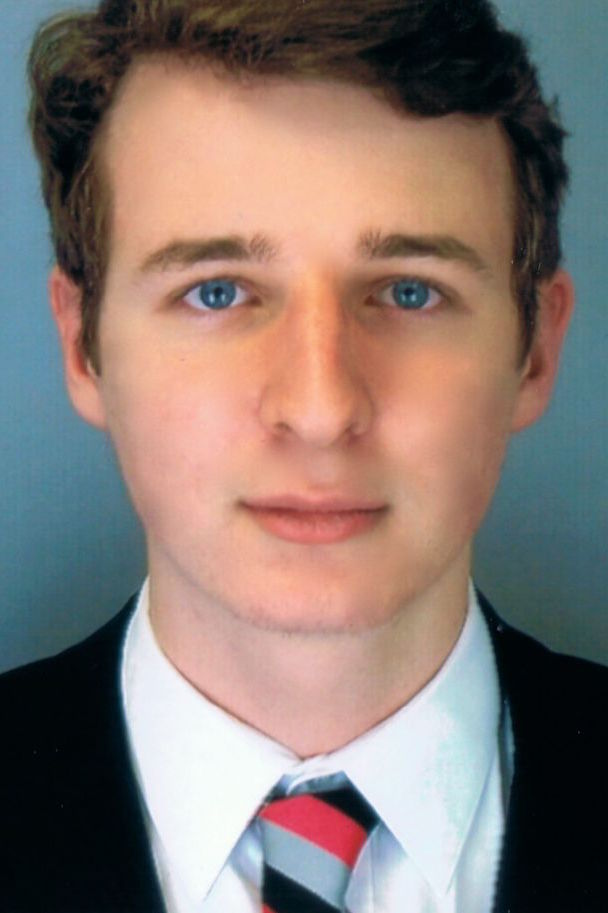
\includegraphics[height=0.3\textheight]{Files/SW}
        \caption{Samuel Wright}
    \end{subfigure}
    ~~~~
    \begin{subfigure}[b]{0.45\textwidth}
        \centering
        
\includegraphics[height=0.3\textheight]{Files/LY}
        \caption{Luke Yeo}
    \end{subfigure}\\
    \vspace{0.5cm}
    \begin{subfigure}[b]{\textwidth}
        \centering
        
\includegraphics[height=0.3\textheight]{Files/MF}
        \caption{Dr Martin Artman}
        % \caption{Martin Fry}
    \end{subfigure}
\end{figure}


\end{document}
